%% BioMed_Central_Tex_Template_v1.06
%%                                      %
%  bmc_article.tex            ver: 1.06 %
%                                       %

%%IMPORTANT: do not delete the first line of this template
%%It must be present to enable the BMC Submission system to
%%recognise this template!!

%%%%%%%%%%%%%%%%%%%%%%%%%%%%%%%%%%%%%%%%%
%%                                     %%
%%  LaTeX template for BioMed Central  %%
%%     journal article submissions     %%
%%                                     %%
%%          <8 June 2012>              %%
%%                                     %%
%%                                     %%
%%%%%%%%%%%%%%%%%%%%%%%%%%%%%%%%%%%%%%%%%


%%%%%%%%%%%%%%%%%%%%%%%%%%%%%%%%%%%%%%%%%%%%%%%%%%%%%%%%%%%%%%%%%%%%%
%%                                                                 %%
%% For instructions on how to fill out this Tex template           %%
%% document please refer to Readme.html and the instructions for   %%
%% authors page on the biomed central website                      %%
%% http://www.biomedcentral.com/info/authors/                      %%
%%                                                                 %%
%% Please do not use \input{...} to include other tex files.       %%
%% Submit your LaTeX manuscript as one .tex document.              %%
%%                                                                 %%
%% All additional figures and files should be attached             %%
%% separately and not embedded in the \TeX\ document itself.       %%
%%                                                                 %%
%% BioMed Central currently use the MikTex distribution of         %%
%% TeX for Windows) of TeX and LaTeX.  This is available from      %%
%% http://www.miktex.org                                           %%
%%                                                                 %%
%%%%%%%%%%%%%%%%%%%%%%%%%%%%%%%%%%%%%%%%%%%%%%%%%%%%%%%%%%%%%%%%%%%%%

%%% additional documentclass options:
%  [doublespacing]
%  [linenumbers]   - put the line numbers on margins

%%% loading packages, author definitions

\documentclass[twocolumn]{bmcart}% uncomment this for twocolumn layout and comment line below
%\documentclass{bmcart}

%%% Load packages
\usepackage{amsthm,amsmath}
%\RequirePackage{natbib}
%\RequirePackage[authoryear]{natbib}% uncomment this for author-year bibliography
%\RequirePackage{hyperref}
\usepackage[utf8]{inputenc} %unicode support
%\usepackage[applemac]{inputenc} %applemac support if unicode package fails
%\usepackage[latin1]{inputenc} %UNIX support if unicode package fails
\usepackage{listings}
\lstset{
numbers=left,%positionner les nombres à gauche
tabsize=2, %taille du tableau
frame=single, %un seul frame
breaklines=true, %forcer le retour à la ligne quand trop long
numberstyle=\tiny \bf \color{blue}, %style pour les numéros
stepnumber=1,
numbersep=12pt,
firstnumber=1, %commencer les numéros à 1
basicstyle=\ttfamily,
numberfirstline=true, %numéroter la première ligne
literate={~} {$\sim$}{1} %joli ~ pour faire comme un terminal
}

\usepackage{graphicx}

%%%%%%%%%%%%%%%%%%%%%%%%%%%%%%%%%%%%%%%%%%%%%%%%%
%%                                             %%
%%  If you wish to display your graphics for   %%
%%  your own use using includegraphic or       %%
%%  includegraphics, then comment out the      %%
%%  following two lines of code.               %%
%%  NB: These line *must* be included when     %%
%%  submitting to BMC.                         %%
%%  All figure files must be submitted as      %%
%%  separate graphics through the BMC          %%
%%  submission process, not included in the    %%
%%  submitted article.                         %%
%%                                             %%
%%%%%%%%%%%%%%%%%%%%%%%%%%%%%%%%%%%%%%%%%%%%%%%%%


%\def\includegraphic{}
%\def\includegraphics{}

\newcommand{\Energ}{\ensuremath{{\mathcal E}}}
\newcommand{\Ress}{\ensuremath{{\mathcal A}}}
\newcommand{\Reg}{\ensuremath{{\mathcal R}^{eg}}}
\newcommand{\FPx}{\ensuremath{{\mathcal F}_{px}}}
\newcommand{\ETer}{\ensuremath {\mathcal T}}

%%% Put your definitions there:
\startlocaldefs
\endlocaldefs


%%% Begin ...
\begin{document}

%%% Start of article front matter
\begin{frontmatter}

\begin{fmbox}
\dochead{Software}

%%%%%%%%%%%%%%%%%%%%%%%%%%%%%%%%%%%%%%%%%%%%%%
%%                                          %%
%% Enter the title of your article here     %%
%%                                          %%
%%%%%%%%%%%%%%%%%%%%%%%%%%%%%%%%%%%%%%%%%%%%%%

\title{MicMac -- a free, open-source solution for photogrammetry}

%%%%%%%%%%%%%%%%%%%%%%%%%%%%%%%%%%%%%%%%%%%%%%
%%                                          %%
%% Enter the authors here                   %%
%%                                          %%
%% Specify information, if available,       %%
%% in the form:                             %%
%%   <key>={<id1>,<id2>}                    %%
%%   <key>=                                 %%
%% Comment or delete the keys which are     %%
%% not used. Repeat \author command as much %%
%% as required.                             %%
%%                                          %%
%%%%%%%%%%%%%%%%%%%%%%%%%%%%%%%%%%%%%%%%%%%%%%

%\author[
%   addressref={aff1,aff2},                   % id's of addresses, e.g. {aff1,aff2}
%   corref={aff1},                       % id of corresponding address, if any
%   noteref={n1},                        % id's of article notes, if any
%   email={ewelina.rupnik@ensg.eu}   % email address
%]{\inits{ER}\fnm{Ewelina} \snm{Rupnik}}
%\author[
%   addressref={aff1,aff3},
%   email={?}
%]{\inits{MD}\fnm{Mehdi} \snm{Daakir}}
%\author[
%   addressref={aff1},
%   email={Marc.Pierrot-Deseilligny@ensg.eu}
%]{\inits{MPD}\fnm{Marc} \snm{Pierrot Deseilligny}}
%%%%%%%%%%%%%%%%%%%%%%%%%%%%%%%%%%%%%%%%%%%%%%
%%                                          %%
%% Enter the authors' addresses here        %%
%%                                          %%
%% Repeat \address commands as much as      %%
%% required.                                %%
%%                                          %%
%%%%%%%%%%%%%%%%%%%%%%%%%%%%%%%%%%%%%%%%%%%%%%

%\address[id=aff1]{%                           % unique id
%  \orgname{ENSG, \'Ecole Nationale des Sciences G\'eographiques}, % university, etc
%  %\street{Waterloo Road},                     %
%  %\postcode{}                                % post or zip code
%  \city{Champs-sur-Marne},                              % city
%  \cny{France}                                    % country
%}
%
%\address[id=aff2]{%                           % unique id
%  \orgname{IPGP -- Institut de Physique du Globe de Paris, Sorbonne Paris Cit\'e, Univ Paris Diderot, CNRS}, % university, etc
%  %\street{Waterloo Road},                     %
%  %\postcode{}                                % post or zip code
%  \city{Paris},                              % city
%  \cny{France}                                    % country
%} 
%
%\address[id=aff3]{%
%  \orgname{Vinci-Construction-Terrassement, Sixense Mapping},
% % \street{D\"{u}sternbrooker Weg 20},
% % \postcode{24105}
%  \city{Morangis},
%  \cny{France}
%}
  

%%%%%%%%%%%%%%%%%%%%%%%%%%%%%%%%%%%%%%%%%%%%%%
%%                                          %%
%% Enter short notes here                   %%
%%                                          %%
%% Short notes will be after addresses      %%
%% on first page.                           %%
%%                                          %%
%%%%%%%%%%%%%%%%%%%%%%%%%%%%%%%%%%%%%%%%%%%%%%

\begin{artnotes}
%\note{Sample of title note}     % note to the article
\note[id=n1]{Equal contributor} % note, connected to author
\end{artnotes}

\end{fmbox}% comment this for two column layout

%%%%%%%%%%%%%%%%%%%%%%%%%%%%%%%%%%%%%%%%%%%%%%
%%                                          %%
%% The Abstract begins here                 %%
%%                                          %%
%% Please refer to the Instructions for     %%
%% authors on http://www.biomedcentral.com  %%
%% and include the section headings         %%
%% accordingly for your article type.       %%
%%                                          %%
%%%%%%%%%%%%%%%%%%%%%%%%%%%%%%%%%%%%%%%%%%%%%%

\begin{abstractbox}

\begin{abstract} % abstract
%
The publication familiarizes the reader with {\tt MicMac} -- a free, open-source photogrammetric software for 3D reconstruction. A brief history of the tool, the organisation of the software and its unique features \textit{vis-à-vis} other software tools are in the highlight.\\ 
The essential algorithmic aspects of the \textit{structure from motion} and image dense matching problems are discussed from the implementation and the user's viewpoints. The work finalizes by reviewing the tools which serve to interact with the user, i.e. image measurement, visualization and data conversion tools.  
%
\end{abstract}

%%%%%%%%%%%%%%%%%%%%%%%%%%%%%%%%%%%%%%%%%%%%%%
%%                                          %%
%% The keywords begin here                  %%
%%                                          %%
%% Put each keyword in separate \kwd{}.     %%
%%                                          %%
%%%%%%%%%%%%%%%%%%%%%%%%%%%%%%%%%%%%%%%%%%%%%%

\begin{keyword}
\kwd{free}
\kwd{open-source}
\kwd{photogrammetry}
\kwd{structure from motion}
\kwd{bundle adjustment}
\kwd{semi-global image dense matching} 
\end{keyword}

% MSC classifications codes, if any
%\begin{keyword}[class=AMS]
%\kwd[Primary ]{}
%\kwd{}
%\kwd[; secondary ]{}
%\end{keyword}


\end{abstractbox}
%
%\end{fmbox}% uncomment this for twcolumn layout

\end{frontmatter}

%%%%%%%%%%%%%%%%%%%%%%%%%%%%%%%%%%%%%%%%%%%%%%
%%                                          %%
%% The Main Body begins here                %%
%%                                          %%
%% Please refer to the instructions for     %%
%% authors on:                              %%
%% http://www.biomedcentral.com/info/authors%%
%% and include the section headings         %%
%% accordingly for your article type.       %%
%%                                          %%
%% See the Results and Discussion section   %%
%% for details on how to create sub-sections%%
%%                                          %%
%% use \cite{...} to cite references        %%
%%  \cite{koon} and                         %%
%%  \cite{oreg,khar,zvai,xjon,schn,pond}    %%
%%  \nocite{smith,marg,hunn,advi,koha,mouse}%%
%%                                          %%
%%%%%%%%%%%%%%%%%%%%%%%%%%%%%%%%%%%%%%%%%%%%%%

%%%%%%%%%%%%%%%%%%%%%%%%% start of article main body
% <put your article body there>

%
%Since this type of article introduces the framework, system architecture and functionalities of a certain software/service and there is less research innovation involved, the articles of this type could be as short as 5 pages including tables and figures.
%
%
%Interested to see an example of such an article? Very recently, the first "software article" of our journal was published. Please check it using the link below:
%
%
%http://opengeospatialdata.springeropen.com/track/pdf/10.1186/s40965-016-0008-x?site=opengeospatialdata.springeropen.com

%%%%%%%%%%%%%%%%
%% Background %%
%%
\section*{Introduction}
Photogrammetry is the art, science, and technology of obtaining geometric information on the 3-dimensional shape and orientation of objects from photographs and other imaging sensors. It is a cheap measurement methodology as it can be executed by practically any digital camera of a decent make. It is instantaneous as it captures the observed phenomena at once and in a split second. It is automated to a high degree due to the advent of the digital era and the rapid developments in automated data processing, hence accessible to non-expert users. The milestones that rejuvenated photogrammetry, brought it forward and placed among other competitive remote sensing techniques (e.g. Light Detection and Ranging LiDAR) merits to the discipline of computer vision \cite{granshaw2015editorial}. Among several milestones leading to this progress are the automated interest points detection \cite{Lowe2004}, the \textit{Structure from Motion} (\textit{SfM}) algorithms capable of reconstructing scenes from sets of unordered image collections \cite{snavely2006photo,marc:11:apero}, and the dense image matching techniques delivering surface models of resolution equal to the pixel size on the ground \cite{pierrot2006multiresolution}, \cite{hirschmuller2008stereo}.\par
%
%\cite{ressl2016dense}
All this contributes to an ever growing visibility of the photogrammetric tools across various fields of science and engineering, the growing market interest, and subsequently a multitude of photogrammetric/computer vision libraries and software solutions, be it commercial or free/open-source. {\tt MicMac} -- together with \textit{Bundler}, \textit{PMVS}, \textit{VisualSfM}, \textit{OpenCV}  and others -- belongs to the open-source solutions. This publication aims at familiarizing the reader with the philosophy behind {\tt MicMac}, some of its crucial algorithmic aspects, the software architecture and the pool of available tools. The paper is organised as follows ....
 
%  
% 
%
%


 
\subsection*{Historical notes}
{\tt MicMac} has been developed at the \textit{National Institute of Geographic and Forestry Information} (IGN) and the \textit{National School of Geographic Sciences} (ENSG), since 2003. Initially, the software tools were developed having in mind exclusively the IGN's cartographic production. The independent tools were interfaced in 2005 via an XML framework, allowing the user to freely parametrize the calculations at all processing stages. In 2007, IGN began to freely distribute {\tt MicMac} under the CECILL-B license that is a version of the L-GPL license adapted to the french law.  Until 2008, the dense image matching of already oriented images was possible only with the IGN's internal image file format. In the same year the {\tt Apero} tool was added to the sofware kernel, offering from now on the possibility to estimate camera exterior and interior orientations, with no restriction on the formatting. In 2010, the XML interface was replaced by a simplified command line. This evolution contributed to an improved accessibility, diffusion and subsequently a better visibility of the software in the scientific communities, and the general public.\par
From 2010 on, {\tt MicMac} has undergone significant evolution due to its implication in many french and european-based projects. On top of the scientific contributions to the source code, the additional funding brought about sofware distributions under Windows, Mac OSX, as well as the GPU processing for certain tasks (e.g. multi-image correlation, optimization with dynamic programming).

\subsection*{{\tt MicMac} \textit{vis-à-vis} other tools}
%The philosophy and software architecture
From the architecture point of view, the unique feature of {\tt MicMac} with respect to its alternatives is that the user can operate on different software {levels}, c.f. Fig.~\ref{fig:architecture}. The least experienced user can steer the processing by a simple command line where little or no parameters must be set. A user with a good command of photogrammetry can operate from the same command line by adapting the parameters typically filled with default values. An expert user can have access to every single parameter at any processing step via a set of XML files (cf. Fig.~\ref{fig:architecture}). On top of that, developers and scientists can use {\tt MicMac} as a library, implement their own algorithms, and share them for the benefit of photogrammetric community. This said, {\tt MicMac} was designed primarily as a tool for professionals and consequently is far from a model design in the sense of HCI~\footnote{\textit{Human-computer interaction}}.\par 
%
{\tt MicMac}, as a photogrammetric tool, stresses the metrological aspect of the reconstruction problem, and provides tools typically unavailable in existing software alternatives, for instance:
\begin{itemize}
\item access to intermediary results in open data formats allowing to interact with the processing chain at any desired stage,
\item qualitative evaluation of the results via quality indicators (e.g. bundle adjustment residuals, covariance matrices, parameter's sensitivity, correlation images),
\item a wide range of camera calibration models,
\item two-dimensional dense image matching for deformation studies,
\item processing of frame cameras and pushbroom sensors,
\item processing of scanned analogue images,
\item architecture adapted to big datasets.
\end{itemize}
%
%
\subsection*{Software organisation}
{\tt MicMac} is organised in a number of modules, accessible through a common command {\tt mm3d}. Execution with a unique command has a twofold advantage of (a) allowing for factorization of certain developments while keeping the the binary files compact, and from the point of view of a user, (b) it is easy to remember giving instantaneous access to all modules. For instance, typing the {\tt mm3d} will print the list of the modules at the disposal, c.f. Fig.~\ref{fig:help}.
%
Invoking a selected module is followed by a number of parameters. The obligatory parameters must be specified at first and since they do not carry names, their order of occurrence is important. In the example shown in Fig.~\ref{fig:help}, the obligatory parameter would be the format specification, and the change coordinate file {\tt ChSys} serves as an option.


\section*{The algorithmic aspects}
The photogrammetric workflow encompasses the passage from images, through the estimation of the orientation parameters, all the way to a 3D surface model. In other words, it is a passage from a 2D representation of the world captured by a camera, through inference of the position and rotation of that camera at the moment of the image taking, towards a 3D restitution of the lost dimension. As long as the quality of the final output depends on the skillful engineering of many small processing steps, estimation of the camera orientation parameters and the matching algorithms constitute the heart of the pipeline. Respectively, the coming sections concentrate on these two aspects, report on the adopted methods and give a global look on what is possible in {\tt MicMac}.

 

\subsection*{Structure from motion}
Recovery of the structure (i.e. 3D coordinates of the observed scene) and the motion (i.e. the camera interior and exterior orientation parameters) is essentially an estimation problem, where the imaging equation constitutes the model. It is well known that this model (i.e. the transformation from 3D to 2D space and vice-versa also referred to as collinearity equation) is not linear, hence requires linearization. Moreover, there exists no direct algorithm able to compute orientation parameters globally consistent with a number of images (generally $n>3$). To overcome this gap, bootstrap solutions were proposed. Using direct algorithms for a single image, a pair or triplet of images, the global orientation is deduced sequentially~\cite{snavely2006photo} or hierarchically~\cite{toldo2015hierarchical} starting from a seed image pair. The so-obtained parameters serve as input to a system of equations composed of the linearized collinearity equations, where their optimal values -- in the stochastic sense -- are found iteratively. The observations (e.g. tie points) are redundant therefore the solution is deduced with the least squares method by minimizing an objective function. The typical function is the squared differences between the nominal observations and those predicted from the estimated model%(i.e. based on the current parameter estimates)
, possibly subject to constraints. The latter stage is also known as the bundle adjustment (BA).\par 
%
\paragraph*{MicMac implementation. }
%
{$\:${ \tt MicMac}} solves the BA with the Levenberg-Marquardt (L-M) method. The L-M is in essence the Gauss-Newton method enriched with a damping factor to handle rank-deficient (or nearly so) Jacobian matrices~\cite{nocedal2006numerical}. A range of different observations equations, constraints and unknowns (i.e. parameters) are allowed in the adjustment routine, among them:
\begin{itemize}
\item tie points (adjustment with points),
\item lines (adjustment with lines; added in the context of georeferencing aerial photographs with a 3D database of roads),
\item perspective centers derived from direct georeferencing (i.e. GNSS),
\item ground control points (GCP),
\item the lever-arm vector separating the GNSS antenna and the perspective center,
\item rigid relative orientation between cameras (i.e. the rigid block; useful for multi-camera systems)
\end{itemize}
%
On top of that, a broad spectrum of camera calibration models are accessible. Both argumentation are supported, the physical and the phenomenological. The former models any imaging error attributed to a phenomenon of a physical nature, while the latter models solely the effects of the lens imperfections, without interrogating its causes. The total distortion is defined as a composition of predefined elementary distortions, such as radial, decentric, polynomial, fish-eye etc., however, typically the major distortion are modeled by the physical model, while the polynomial models remove the less significant remaining systematism.\par 
%
The critical element of the BA's mathematical model is the observation weighting, known as the stochastic model. {\tt MicMac} specifies three different weighting strategies. The first strategy corresponds to the weighting in the classical model known in photogrammetry -- the Gauss-Markov -- where the observations are weighted by their true standard deviations known \textit{a priori}. The second strategy controls the influence of a particular category of observations so as to avoid solutions that are driven by a single category only for the sheer reason of its abundant observations. The last strategy addresses the robustness. The weight is a function of the observation's residual in the BA, therefore giving more credibility to observations that are close to the model being estimated, and contrary, limiting the influence of observations with high residuals.
%
\paragraph*{User's viewpoint.}
There are two principal modules that handle the camera orientation recovery with the simplified interface -- {\tt Tapas}, {\tt Campari} -- and either of the modules calls the \textit{parent} orientation tool {\tt Apero} (cf. Fig.~\ref{fig:architecture}). {\tt Tapas} calculates the purely relative orientation of images, using observed tie points as the only input. Since at this point there is no \textit{a priori} on positions and rotations of the cameras, {\tt Tapas}  also entails the initialization step where it progressively reconstructs the cameras with the help of the direct orientation algorithms, and intertwines it with the BA routine. \par 
%
Unlike in {\tt Tapas}, {\tt Campari} is a BA module adapted to handling heterogeneous observations. Besides the tie points, it works with GCPs, the GNNS data and can impose various constraints on the solution. This module is typically executed once a good relative orientation has been established, and, all input data shall be defined in a consistent coordinate system (CS). To bring the cameras' relative orientation to the same CS of e.g. the GCPs, a module performing spatial similarity transformation (e.g. {\tt GCPBascule}; c.f. Fig.~\ref{fig:architecture}) must be evoked beforehand. Both, {\tt Campari} and all variations of the  {\tt Bascule} can be regarded as georeferencing tools.\par 
%
Since recently, {\tt MicMac} provides the user with the internal accuracy estimates of the BA parameters (their standard deviations and correlations) derived from covariance matrices.

\subsection*{Multi-view stereo image matching (MVSM)}%or multi-view stereo image matching
%
Given several overlapping images with known orientation parameters, MVSM is the process of reconstructing a complete 3D model of the scene by finding corresponding pixels (i.e. their disparities or depths, respectively) between image pairs, and triangulating them in space. The generic algorithm is defined as an energy minimization problem that searches for a disparity map that minimizes the energy. The minimization can be solved with local, semi-global and global algorithms. Today the golden standard method for producing dense 3D models from images is the semi-global matching~\cite{hirschmuller2008stereo}.\par
%Within all local algorithms the disparity at a given point depends only on the finite window around that point, whereas the global algorithms simultaneously solve for the entire disparity map that is globally consistent with an implicit smoothness constraints. Today the golden standard method for producing dense 3D models from images is the semi-global matching~\cite{hirschmuller2008stereo}.\par 
%
Image matching breaks down into three processing stages: computation of the pixel matching cost, cost aggregation and disparity calculation. The matching cost is a measure of similarity, i.e. describes the likelihood that two pixels do belong to a unique point in 3D. %This measure must be designed robust and insensitive to radiometric differences and noise. The most common similarity measures are normalized cross-correlation, Census, mutual information, absolute intensity differences~\cite{hirschmuller2009evaluation} and very recently also trained and subsequently predicted matching costs~\cite{zbontar2015computing}.
As the matching can be ambiguous, and the minimum cost insignificant, an additional \textit{a priori} is imposed on the energy function that penalizes changes in disparities of neighboring pixels (the case of local and semi-global algorithms). This aggregation takes place within a window, a 1D path (locally) or multiple paths (semi-globally). In the latter case, the cost for a given disparity is an accumulated cost along many paths that end in the pixel in question~\cite{szeliski2010computer}.
%
\paragraph*{MicMac implementation}
%
Image dense matching in {\tt MicMac} is possible with a semi-global and global algorithms. The objective of matching is to find a mapping $\mathcal{F}_{px}$ from the space $\tau$ where the depth is computed, to the disparity space $\varepsilon_{px}$. Depending on the restitution geometry, the $\tau$ can be the 3D euclidean space or the image space of the master image, while the $\varepsilon_{px}$ can be either the disparity or the depth of the 3D~euclidean~$\mathcal{Z}$.\par  
%
The motivation to distinguish between these two restitution geometries -- the ground and the image -- is twofold. On the one hand, a Digital Surface Models (DSM) produced from aerial images is normally defined in some reference CS, therefore it is more intuitive to perform the reconstruction directly in the target CS (i.e. ground geometry; alternatively one can use an arbitrary CS and transform the result \textit{a posteriori}), where the disparity space $\varepsilon_{px}$ is the euclidean $\mathcal{Z}$ (cf. Fig.~\ref{fig:matchGeom}(A)). 
On the other hand, it is known that matching in image space with a master and a set of slaves images is more reliable, especially in close-range photogrammetry applications and for small datasets. The disparity space $\varepsilon_{px}$ in the image geometry is then either the depth along the ray or the respective disparity in image space (i.e. the image geometry; cf. Fig.~\ref{fig:matchGeom}(B) and \ref{fig:matchGeom}(C)). It is up to the user which geometry to employ.
\par
%
{\tt MicMac} offers a very flexible formulation of the matching cost function as far as its terms, the optimization algorithm and the dimension of the matching are regarded (cf. Eq.~\ref{eq:energy}).   
%\begin{equation}
%\begin{split}
%   E(Z) = \sum C(i,j,Z(i,j)) \\+
%   F(|Z(i+1,j)-Z(i,j)|)  + \dots\label{eq:energy}
%\end{split}
%\end{equation}
\begin{equation}
\label{eq:energy}
   \Energ(\FPx) = \iint_\ETer \Ress(x,y,\FPx(x,y)) + \| \nabla(\FPx) \|^{reg}
\end{equation}
\begin{equation}
\label{eq:energySmoothTerm}
   \| \nabla(\FPx) \|^{reg} = \alpha_1*|\nabla(\FPx^1)|+\alpha_2*|\nabla(\FPx^2)|
\end{equation}

where\\
$\Ress(x,y,\FPx(x,y))$ is the measure of similarity between pixels with $\Ress=0$ when they are identical; $\| \nabla(\FPx) \|^{reg}$ a norm on the gradient, which is used as
 a regularity criteria (it penalizes the variation of \FPx); $\alpha_1$ is the regularization on first component of disparity and $\alpha_2$ the regularization  on the second component (equivalent of matching in the direction transverse to the epipolar line).\par 
%
\vspace{0.5cm}
The $\| \nabla(\FPx) \|^{reg}$ controls the \textit{a priori} on the disparity space in a way that:

\begin{itemize}
   \item  if the desired model is smooth, a convex  function~$F$  is adequate (it's better to
          climb a given jump by regular step),

   \item  if  the desired model has many discontinuities, a concave function~$F$ is adequate
          (it's better to climb a given jump in one single step),

   \item when there is no strong prior, the  default choice is to have $F$ linear,

   \item if \textit{a priori} knowledge on scene slope exists, it can impose an allowable maximum scene slope,
   \item for 2D matching, non-isotropic smoothing factors can be set. 
\end{itemize}
%
The actual similarity measure $\Ress(x,y,\FPx(x,y))$ is the normalized cross correlation coefficient, defined as a function of multiple images, rather than a single pair. The coefficient can privilege an image out of a set of images (e.g. a master image), or consider the set as "symmetrical". Varying cross correlation window sizes and weighted windows are also possible.\par 
%
To find the disparity map that minimizes the energy, {\tt MicMac} by default employs a multi-directional variant of the dynamic programming algorithm. The results along independent directions are aggregated by taking a mean of all results or simply the best result. Optionally, a global minimization by the Min-Cut/Max-Flow algorithm~\cite{roy1998maximum} can be enforced.\par 
%
In order to limit the disparity search-space, speed up the calculation and to reduce the noise,  {\tt MicMac} adopts a multi-resolution matching approach where coarse resolution disparity maps serve as predictors of the fine resolution output.\par 
% 
%guesswork

\paragraph*{User's viewpoint}
DSM creation in {\tt MicMac} takes places via several tools that are semi- or fully-automated. In both cases the \textit{parent} tool to handle the low-level dense matching is the {\tt MicMac}, which an expert user can access via an XML file.\par 
%
{\tt Malt}, the semi-automated tool operates in three predefined modes, i.e. {\tt Ortho}, {\tt UrbanMNE} and {\tt GeomImage} that are adapted to producing orthophotography, urban DSMs in ground geometries and DSMs in image geometry. Accordingly, {\tt Ortho} and {\tt UrbanMNE} would be used for flat terrains or planar surfaces (i.e. 2.5D; c.f. Fig.~\ref{fig:basRelief}, \ref{FIG:OK:Concrete}, \ref{FIG:Mubich:PxTr}) whereas {\tt GeomImage} is more suitable for true 3D surfaces (c.f. Fig.~\ref{fig:fisheye}).\par 
%
The inconvenience of the {\tt Malt GeomImage} is that for a complete 3D restitution of a surface, one must indicate several master and their relevant slave images. As long as for simple object geometries it is feasible, it becomes inefficient for more complex and extensive objects. The fully automated tools overcome this impediment by making this choice for the user, while prioritising completeness and precision of the output. The two automated tools are {\tt C3DC} and {\tt PIMs} which furnish a point cloud and a set of depth maps, respectively. To proceed with the orthophotomap generation, the {\tt PIMs2MNT} and subsequently the {\tt Tawny} shall be executed (an exemplar orthophoto in Fig.~\ref{fig:fortress}). The latter collects the per-image orthophotos and merges it to a single mosaic. The individual orthophotos can be created either by {\tt PIMs2MNT} tool or {\tt Malt}; c.f. Fig.~\ref{fig:architecture}.\par 
%
Besides the classical 1D matching (along an image ray, an image row or the Z-coordinate) for reconstruction of object geometry , {\tt MicMac} also implements a 2D matching strategy. This strategy is useful in 2D deformation studies between rectified images (c.f. Fig.~\ref{FIG:OK:Concrete}; also {\tt MM2DPosSism}), as an orientation quality estimation tool to asses the remaining y-parallax ({\tt MMTestOrient}; c.f. Fig.~\ref{FIG:Mubich:PxTr}), or in cases when orientation parameters are unknown or known with poor precision (executed with XML file). Because the expected disparities pertinent to geometry are of higher frequencies than those along the y-parallax, the regularization of the energy function in the two direction is managed separately; c.f. Eq.~\eqref{eq:energySmoothTerm}.\par 
%
Lastly, in the event when all camera optical centers are located on a 3D line, parallel to the surveyed object, and the reconstruction is defined in object space, the matching becomes ambiguous along the epipolar lines. To avoid the ambiguities and the resultant noise, {\tt MicMac} calculates the matching in ortho-cylindrical coordinates (see {\tt RepLocBascule}). 

\section*{Interactive tools}
Although {\tt MicMac} by default is based on simplified command lines, for some processes (e.g. image measurements, visualization of the results)  it is more straight-forward to have a graphical user interface. In this section the different user-interaction interfaces available in {\tt MicMac} are presented. Besides this, for multiple commands there exists a graphical user interface that replaces the standard command line. To run it, the user should simply type the name of the command preceded by the letter 'v'. For example, in the {\tt GrShade} command presented below, the user can type {\tt vGrShade} and a visual interface (c.f. Fig  \ref{fig:visuInterfaceV}) appears and used to run the command.\par 
%
All results produced by {\tt MicMac} are exclusively in open data formats (tif, xml, ply) and as such it opens up the possibility to interact with the processing chain at any desirable stage. For instance, the user can import interior and exterior image orientation data and proceed with the dense matching and orthophoto generation. Or vice versa, the orientation parameters or epipolar images can be generated to proceed with an alternative image dense matcher. The reader is advised to refer to the software documentation~\cite{micmac:manual} for more details on the conversion procedures. 
 
\subsection*{Image measurement tools}
In the following, several tools for image measurements and the input of 2D/3D masks are discussed.

Many of the interactive tools are available in a version requiring the installation of {\tt QT} and are available on all platforms. For example, for the {\tt SaisieMasq}, the corresponding QT tool is the {\tt SaisieMasqQT}. Either way, the masking works by creating a binary mask image from a polygonal section in the displayed image, and as such it can be used to, e.g., remove tie points outside the area of the mask (c.f. {\tt HomolFilterMasq}), or to limit the dense reconstruction to a selected part. Moreover, there exists a 3D generalization of the tool where the 3D mask does segmenting of a point cloud by, again, drawing a polygon (c.f. Fig. \ref{fig:saisieMasq}).  This information is then stored in order to be introduced in later processing stages.\par 
% 
The {\tt SaisieAppuisInitQT}/ {\tt Saisie\-AppuisPredicQT} tools allow for measurements of GCPs in the images (c.f. Fig \ref{fig:SaisieGCP}). Provided that the camera orientation parameters are known with a reasonable accuracy, while the GPCs are expressed in the same CS, the latter tool predicts the points image positions to facilitate the measurements step. Measurements necessary to perform a spatial similarity transformation, i.e. the origin, the axes directions and distances, can be collected within another georeferencing tool -- the {\tt SaisieBascQT}. These tools normally precede the georeferencing operations with {\tt GCPBascule} and/or {\tt Campari}. 

\subsection*{Visualization tools}
To visualize the intermediary and final results {\tt MicMac} offers a range of different tools.\par 
%
The {\tt SEL} tool allows to visualize the tie points between a stereo pair calculated by {\tt Tapioca}. The {\tt AperiCloud} tool converts the result of the BA, that is the poses and 3D tie points, to the point cloud ply format.%  (c.f. Fig \ref{fig:apericloud}). 

The {\tt Vino} tool is a simple image viewer adapted to efficient visualization of very large images (i.e. in size of a few gigabytes), irrespective of their type (i.e. integer, float or $>$8Bit). Moreover, it lets the user to modify the histogram of the image or generate an image crop.

Other tools allow a more intuitive visualization of the depth map. For instance, the {\tt to8bits} tool converts 32-bit or 16-bit images to 8-bit images, while the {\tt GrShade} tool computes shading from a depth map image (c.f. Fig \ref{fig:basRelief}). Lastly, the {\tt Nuage2Ply} allows to transform a depth map into a point cloud ply format (c.f. Fig \ref{fig:fisheye}).

\section*{Concluding remarks}
%
{\tt MicMac} is an open-source project for photogrammetry. As the research implementation platform, it serves the IGN's internal needs as well as aims at bringing the state-of-the art 3D image processing algorithms to a wider audience, be it universities, public institutions or enterprises. Like any other open-source project, {\tt MicMac} authorizes the volunteers to contribute or change the source code according to their needs. For more information please refer to:
\begin{itemize}
\item http://micmac.ensg.eu, as the  software's reference webpage;
\item http://forum-micmac.forumprod.com/, for technical support;
\item https://github.com/micmacIGN/, for the source code.
\end{itemize}  
 
 

%%%%%%%%%%%%%%%%%%%%%%%%%%%%%%%%%%%%%%%%%%%%%%
%%                                          %%
%% Backmatter begins here                   %%
%%                                          %%
%%%%%%%%%%%%%%%%%%%%%%%%%%%%%%%%%%%%%%%%%%%%%%

\begin{backmatter}

\section*{Competing interests}
  The authors declare that they have no competing interests.

%\section*{Author's contributions}
%    Text for this section \ldots

%\section*{Acknowledgements}
%  Text for this section \ldots
%%%%%%%%%%%%%%%%%%%%%%%%%%%%%%%%%%%%%%%%%%%%%%%%%%%%%%%%%%%%%
%%                  The Bibliography                       %%
%%                                                         %%
%%  Bmc_mathpys.bst  will be used to                       %%
%%  create a .BBL file for submission.                     %%
%%  After submission of the .TEX file,                     %%
%%  you will be prompted to submit your .BBL file.         %%
%%                                                         %%
%%                                                         %%
%%  Note that the displayed Bibliography will not          %%
%%  necessarily be rendered by Latex exactly as specified  %%
%%  in the online Instructions for Authors.                %%
%%                                                         %%
%%%%%%%%%%%%%%%%%%%%%%%%%%%%%%%%%%%%%%%%%%%%%%%%%%%%%%%%%%%%%

% if your bibliography is in bibtex format, use those commands:
\bibliographystyle{bmc-mathphys} % Style BST file (bmc-mathphys, vancouver, spbasic).
\bibliography{biblio}      % Bibliography file (usually '*.bib' )
% for author-year bibliography (bmc-mathphys or spbasic)
% a) write to bib file (bmc-mathphys only)
% @settings{label, options="nameyear"}
% b) uncomment next line
%\nocite{label}

% or include bibliography directly:
% \begin{thebibliography}
% \bibitem{b1}
% \end{thebibliography}

%%%%%%%%%%%%%%%%%%%%%%%%%%%%%%%%%%%
%%                               %%
%% Figures                       %%
%%                               %%
%% NB: this is for captions and  %%
%% Titles. All graphics must be  %%
%% submitted separately and NOT  %%
%% included in the Tex document  %%
%%                               %%
%%%%%%%%%%%%%%%%%%%%%%%%%%%%%%%%%%%

%%
%% Do not use \listoffigures as most will included as separate files

\section*{Figures}
%
\begin{figure*}
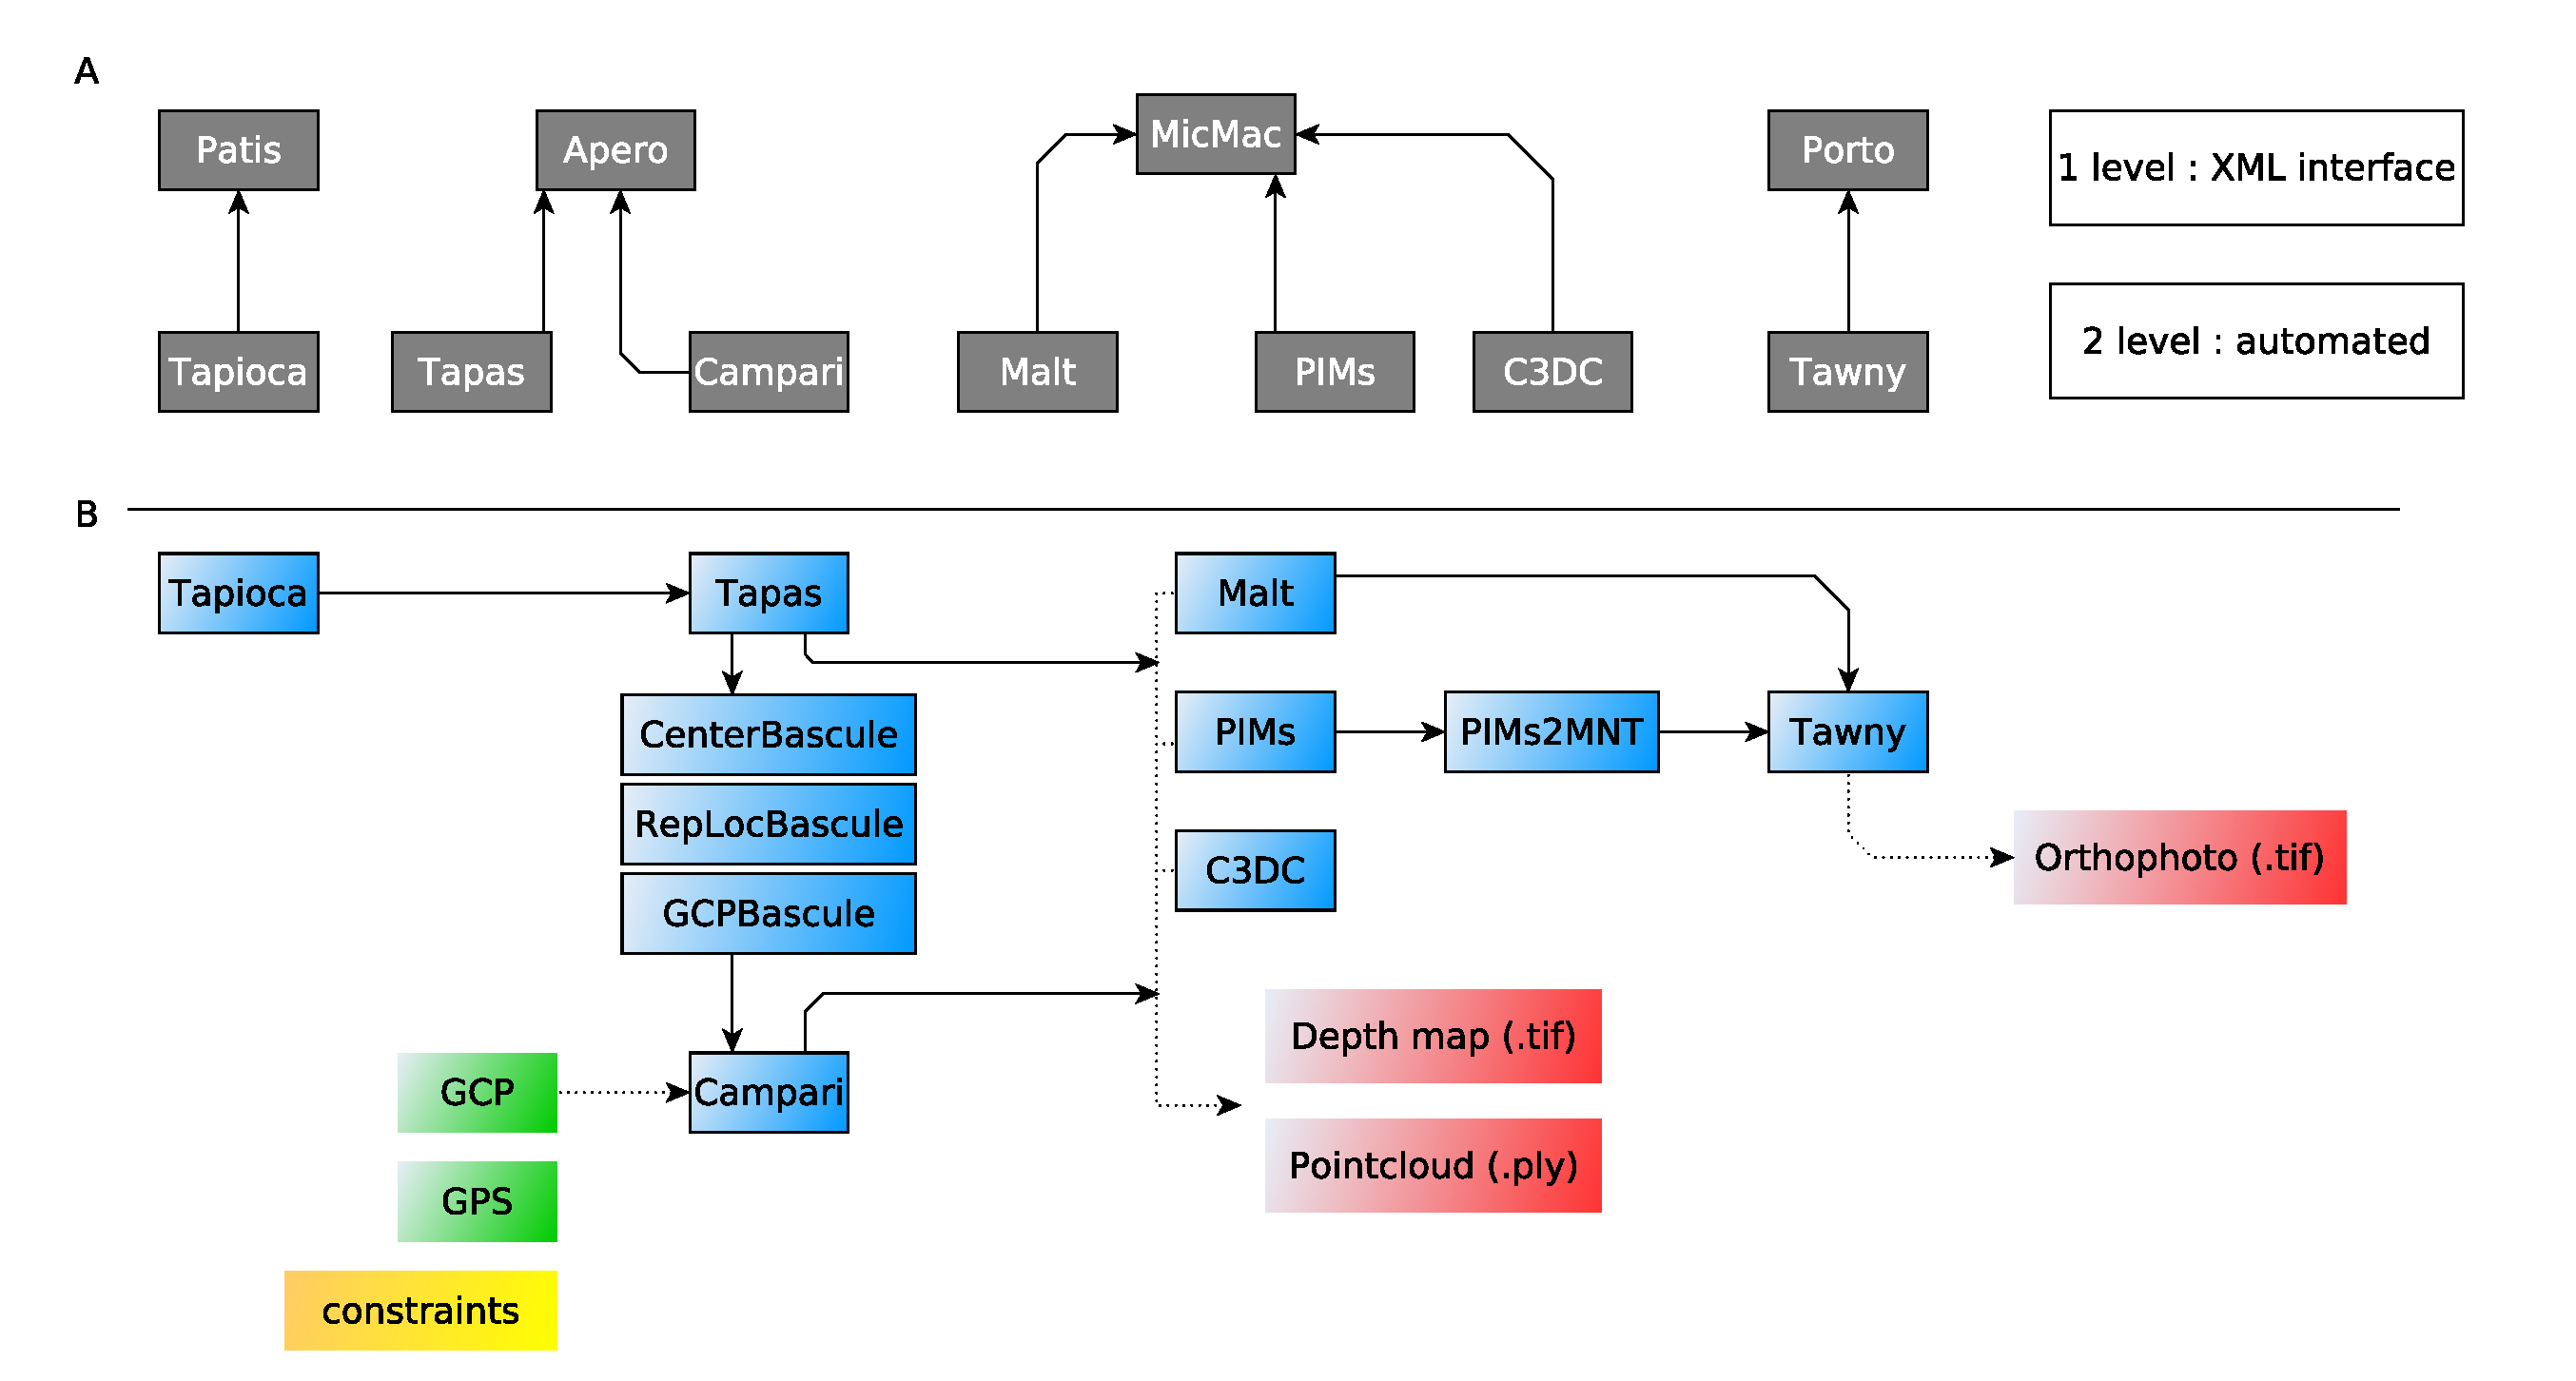
\includegraphics[width=2\linewidth]{img/architecture.pdf}\caption{The simplified architecture of the core {\tt MicMac} modules. (A) the low-level and high-level modules dependencies, (B) the processing workflow. Marked in red are the outcome products, in green are the direct georeferencing inputs. }\label{fig:architecture}
\end{figure*}
% 
\begin{figure*}
\includegraphics[width=2\linewidth]{img/DIM_scenarios.pdf}\caption{Three restitution geometries in {\tt MicMac}. (A) ground, euclidean space, (B) image geometry discretised along the ray, no resampling (C) image space resampled to epipolar geometry. For a range of the potential Z-coordinates/depths/disparities the similarity measure is computed and further passed to the energy minimization solver.}\label{fig:matchGeom}
\end{figure*}
%% 
%\footnotesize
%\begin{figure}[h!]
%\begin{lstlisting}[language=bash,frame=none]
%:~$ mm3d
%mm3d : Allowed commands 
%AllDev		 Force devlopment of all tif/xif
%Ann	 		 Matches points of interest
%AperiCloud	 Visualization of camera in ply
%Apero	 	 Compute external/internal orientations
%BatchFDC	 Tool for batching a set of commands
% ...
%\end{lstlisting}
%\caption{ {{\tt mm3d} is the common command that invokes all {\tt MicMac} modules and their brief description.}}\label{fig:mm3d}
%\end{figure}
%
\footnotesize
\begin{figure}[h!]
\begin{lstlisting}[language=bash,frame=none]
:~$ mm3d OriConvert -help
*****************************
*  Help for Elise Arg main  *
*****************************
Mandatory unnamed args : 
  * string :: {Format specification}
  * string :: {Orientation file}
  * string :: {Targeted orientation}
Named args : 
  * [Name=ChSys] string :: {Change coordinate file}
  * [Name=Calib] string :: {External XML calibration file}
  * [Name=AddCalib] bool :: {Try to add calibration, def=true}
  ...
\end{lstlisting}
\caption{ {Each module is executed with some obligatory and optional parameters. Adding {\tt -help} at the end will print out the expected input arguments}.}\label{fig:help}
\end{figure}

\begin{figure*}
 \begin{tabular}{c c c} 
 \includegraphics[height=50mm]{../../FIGS/SAMPLES/Aj2.jpg} &
 \includegraphics[height=50mm]{../../FIGS/SAMPLES/Aj1.jpg} &
  \end{tabular}
 \caption{{Indoor architecture: } Chapelle imperiale Ajaccio, with 100 fish-eye images;
 left: retrieved camera poses, right: 3D model.}\label{fig:fisheye}
 \end{figure*}

\begin{figure*}
 \begin{tabular}{c c c} 
    \includegraphics[height=34mm]{../../FIGS/SAMPLES/Hiero1_2908.JPG} &
    \includegraphics[height=34mm]{../../FIGS/SAMPLES/Hiero2_2908.JPG} &
    \includegraphics[height=34mm]{../../FIGS/SAMPLES/Hiero3_2908.JPG} 
 \end{tabular}
 \caption{{ Bas Relief} stone in Louvre: the image and the 3D model rendered in shading and depth map.}\label{fig:basRelief}
 \end{figure*}


%
\begin{figure*}
 \begin{tabular}{c c c} 
 \includegraphics[height=40mm]{img/saisieMasq.png} &
 \includegraphics[height=40mm]{../../FIGS/Viabon/masq3d.png} &
  \end{tabular}
 \caption{ Left: drawing of a 2D mask on an image; right: and a 3D mask in a point cloud.}\label{fig:saisieMasq}
 \end{figure*}
%

\begin{figure*}
\begin{center}
 \includegraphics[width=74mm]{../../FIGS/Beton/IM1.jpg}
 \includegraphics[width=56mm]{../../FIGS/Beton/IMCROP.jpg}
 
 \includegraphics[width=65mm]{../../FIGS/Beton/Px1.jpg}
 \includegraphics[width=65mm]{../../FIGS/Beton/Px2.jpg}
 
 \end{center}
 \caption{Under induced force the concrete beam deformed, while a still camera measured the displacements in during the breaking phase. Upper left: the full view image, upper right: a close-up of the concrete structure, bottom left: displacement in the x-coordinate (max amplitude $\frac{1}{4}$ pixel), bottom right:  displacement in the y-coordinate (max amplitude $\frac{1}{4}$ pixel)} 
 \label{FIG:OK:Concrete}
\end{figure*}

\begin{figure*}
 \begin{tabular}{c c}
 \includegraphics[width=80 mm]{../../FIGS/SAMPLES/Salse2.jpg}&
 \includegraphics[width=80 mm]{../../FIGS/SAMPLES/Ortho-Test-Redr.jpg} 
  \end{tabular}
 \caption{Forteresse de Salses, photo acquired from a drone, in collaboration
 with Map-CNRS/ Left: hypsometry and shading maps overlapped, right: an orthophotography.}\label{fig:fortress}
 \end{figure*}


  \begin{figure*}
  \begin{center}
  \includegraphics[height=80mm]{../../FIGS/TestOri/Mun1.jpg}
  \includegraphics[height=80mm]{../../FIGS/TestOri/Mun2.jpg}
  \end{center}
  \caption{Munich dataset, acquired with a DMC camera at GSD of $10$ cm. Left: the depth map, right: the y-parallax generated with {\tt MMTestOrient}. The amplitude of transverse parallax is $\pm\, 0.1$ pixel
  }
  \label{FIG:Mubich:PxTr}
  \end{figure*}

\begin{figure}
 \includegraphics[width=0.8\linewidth]{../../FIGS/Saisie/Visual.jpg}
 \caption{Graphical interface to launch commands}\label{fig:visuInterfaceV}
 \end{figure}
%
\begin{figure}
 \includegraphics[width=0.9\linewidth]{../../FIGS/Saisie/SaisieAppuisInitQT.jpg}
 \caption{Interface for measuring GCPs in images}\label{fig:SaisieGCP}
 \end{figure}
%
%\begin{figure*}
% \begin{tabular}{c c c} 
% \includegraphics[height=25mm]{img/2images.jpg} &
% \includegraphics[height=25mm]{img/sift2images.jpg} &
%  \end{tabular}
% \caption{A stereo pair with corresponding tie points}\label{fig:sel}
% \end{figure*}
 %
%\begin{figure*}
% \begin{tabular}{c c} 
% \includegraphics[height=50mm]{img/chambord_img1.png} &
% \includegraphics[height=50mm]{img/chambord_img2.png}
%  \end{tabular}
% \caption{Export of poses and tie points: terrestrial images (left), terrestrial and aerial images (right)}\label{fig:apericloud}
% \end{figure*}
%
 
%%%%%%%%%%%%%%%%%%%%%%%%%%%%%%%%%%%
%%                               %%
%% Additional Files              %%
%%                               %%
%%%%%%%%%%%%%%%%%%%%%%%%%%%%%%%%%%%

\end{backmatter}
\end{document}
